\section{Section Zero: Introduction}
    \begin{student}
Hello and Welcome to your very first \textsc{PEN Education} \textbf{Mathematics} lesson! Today's topic shall be \underline{Whole Numbers}. But before we begin some context will serve you well:

Each week, you will receive a booklet typeset in this format\footnote{For those curious, the typesetting system is \LaTeX}, we have created approximately 150 such booklets for Math, and another 100 for English. The Mathematics booklets are based off the ICE-EM AMSI Cambridge Textbooks, written by tenured Professors of Mathematics who understand the content and the process of its Education well. If you are ever in the need for further study, or want clarification about a concept beyond what your tutor is able to provide - the textbook is always a fantastic thing to turn to.

Now, the structure of the booklets will always be as follows:
\begin{enumerate}
    \item An \textbf{introduction} to help contextualise the newly learned content with reference to what you have already learned\footnote{in the literature this effective learning principle is termed \emph{elaborative encoding}}
    \item Sectioned \textbf{topics} that each cover \emph{one} important concept. These topics will be listed in the \underline{Table of Contents} on the first page. Use this!
    \item Within each topic will be \textbf{Theory}\footnote{Note that you may not always have a theory section.}, \textbf{Examples} and \textbf{Exercises}
    \item Every question that requires an answer in these booklets will have a corresponding Mark allocated to it. The Marks are tallied in the GradeTable on the last page of every Booklet. Your tutor will mark your work every other week; if the work is not being done you/we should question your place in this tutoring centre. Your marks will be recorded for the statistical analysis.
    \item Each page now has margins inspired by \href{https://tug.ctan.org/macros/latex/contrib/tufte-latex/sample-book.pdf}{Edward Tufte}. Use them to flesh out new ideas as well as write out trivial sums you should know how to do.\reversemarginpar\marginpar{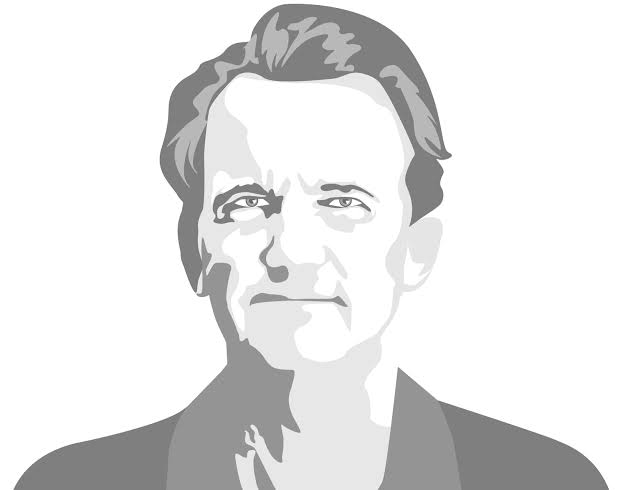
\includegraphics[width=1in]{tufte.jpg}}
    \item Homework:
\end{enumerate}

\subsection{Homework}
The concept of \emph{homework} is so important for us, that I am writing this in its own \emph{subsection}!\tikz[remember picture,overlay,baseline=0pt] \draw[->,thick,gray!50] (0.15,0.05) -- (0.15,1.15);



\smallskip
\fbox{
\fbox{
    \centering
\textsc{\small YOU MUST ATTEMPT ALL HOMEWORK THAT HAS BEEN PRESCRIBED TO YOU.}
}}
\smallskip

This is a law. It must be followed.

Note that, it is not compulsory to \textbf{always} do \textbf{all} of the Homework at the back of the booklet. The only thing that must be done, is the homework you have agreed to do.
It will often be the case that you have other assessment tasks to do. You might have an important Ochestra event to attend, you might have a family holiday planned. You might be sick, you might find it too difficult. All of these are valid --- speak to your tutor about it, they'll \emph{prescribe} you the appropriate amount of homework.

Furthermore, beyond the hurdles of everyday life that might 🛑STOP🛑 you from attempting homework, there is truly great benefit in sitting at home and thinking about the homework problems. You will gain further insight into the tiny little corners of the concepts you have learned. The homework problems have been designed to be slightly harder than the exercises, and the exercises in turn have been designed to be slightly harder than the example questions.

Finally, if you attempt the homework questions, you will be in a \emph{much} better position to score well in the Topic Tests.

\end{student}
\begin{instructor}
Hello and Welcome to the Circus. This Manual is for the instructor, and has been designed to be sparse.

    The pre-conditions for teaching this material is a Band 6 or equivalent in the NESA HSC Advanced Mathematics, and for the English booklets it will be a mid Band 5 and above. The post-conditions for this booklet, i.e. what it guarantees \emph{you}, is \textbf{answers} to all the \textsc{Example}, \textsc{Exercise} and \textsc{Homework Questions}. What it \underline{does not} guarantee you are solutions to the individual questions.

It is expected that you are able to solve all of these via your own volition. It is also expected that you designate homework each week. You may not necessarily be the one to mark it, but you must prescribe it.

    You will also notice that your copy significantly differs from that of the student---you are missing their theory. As a result, your pages numbers are entirely skewed and you should \textbf{not use} page numbers as a guide to find answers within this \textsc{Instructor's Manual}. Furthermore, it would benefit you to read this introduction section before teaching any and every class.

    Ideally, a utopic tutor will not need this \textsc{manual} beyond a cursory reading; s/he should hold a student copy of the booklet throughout class and read out loud the corresponding theory. It will also be of immense benefit for the tutor to delegate paragraphs for the students to read aloud. This will improve their engagement, understanding, reading-comprehension, pronunciation and classroom respect.

    \subsection{Aayush Bajaj}
    I will take a quick moment to introduce myself as my voice will propagate through these booklets. I am a $3^{\text{rd}}$ year Computer Science major at UNSW and went to a selective high school in Sydney. I understand the NESA syllabus well, but these booklets have been designed with the \emph{Australian} curriculum in mind.

    I have been teaching in classroom settings; primary school and high school as well as privately since I graduated in 2019. Since then I have consumed many books on meta-cognition, psychology and evidence-based learning---you will occasionally find references in the footnotes. Furthermore, I apply these to my own studies with great success.

    I typeset these booklets using \LaTeX, compiled with the LuaLatex engine under the \texttt{exam} class. The source code for both \textsc{Instructor} and \textsc{Student} copies lie in the same files and are distinguished by the boolean variable \texttt{printanswers}. For any interested \TeX\ nicians you may send me an email at j@abaj.io, but otherwise, the source code for this project is not available.

    Finally, in the way that Virgil was the guide of Dante Aligheiri---I too shall be your guide for this booklet series. I hope you learn things both from myself and your students, I am certainly learning much in producing these booklets por toi.

    Love,
    AJ
\end{instructor}

    \setcounter{sec0marks}{\thesecmarks}

\section{Section One: Multiplication}
    In the same way that \enquote{to add} is \fillin[to sum], to multiply is to calculate the \fillin[product].

Much in the same way that we \emph{visualised} addition, we are able to visualise multiplication:

\begin{figure}[ht]
    \label{fig:m1}
    \centering
    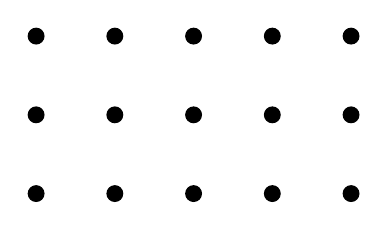
\begin{tikzpicture}
        \foreach \x in {0,1,...,4}
        \foreach \y in {0,1,2}
        \filldraw (\x,\y) circle (0.1);
    \end{tikzpicture}
    \caption{$3\times 5 = 15$ }
\end{figure}

In mathematics, one thing you must reconcile with as early as possible is the fact that 1 concept can be understood, or thought of, in multiple different ways; and each of these ways provides different value. 
For example: multiplication can be conceptualised as addition!

\begin{figure}[ht]
    \label{fig:m2}
    \centering
    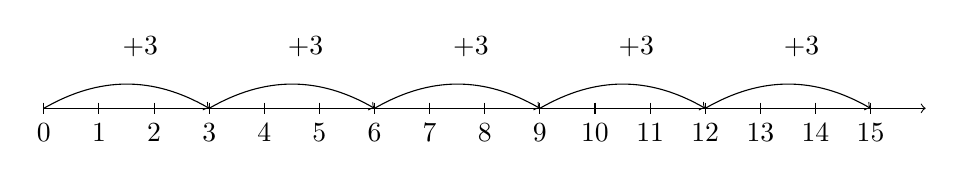
\begin{tikzpicture}[scale=0.7]
        \draw[->] (0,0) -- (16,0);
        \foreach \x in {0,1,...,15}
            \draw[shift={(\x,0)}] (0,3pt) -- (0,-3pt) node[below] {$\x$};
        \foreach \x in {0,3,...,12}
            \draw[->] (\x,0) to[bend left] (3+\x,0) node [above left=15pt] {$+3$};
    \end{tikzpicture}

    \caption{$5\times 3$}
\end{figure}

Note that in the Figure~\ref{fig:m2}, we've demonstrated $5\times 3$ as opposed to the equation we've been thinking about: $3\times 5$. Why is are these 2 the same thing?
\begin{solutionordottedlines}[1in]
    The property of commutativity that we studied in the last lesson, applies to the multiplication operator!
\end{solutionordottedlines}

\fbox{
    \centering
    \parbox{\linewidth}{
        {\large \textbf{Note:} Associativity also applies to multiplication.\[(a\times b)\times c = a \times (b\times c)\]}
}
}

\subsection{Tricks of the Trade}
\subsubsection{Multiplication with 0}
This concept is elementary, but important:

\fbox{
    \centering
\textsc{anything multiplied by 0 is equal to 0}}

\subsubsection{Multiplication by powers of 10}
This is straight-forward---look at how many 0's the power of 10 has, and then just give all those 0's to the other operand\footnote{you should use the space in the margins to define this word if you do not know what it means!}

Thus, $2\times 10$ will just mean I take 1 zero to the 2: $20$. $90\times 1000$ means I take 3 zeros to the $90\,\leadsto\, 90,000$.

\begin{tabular}{lr}
    $2\times 100 =$\fillin[200] & $32\times 10 =\fillin[320]$\\[0.4cm]
    $2\times 1000 = \fillin[2000]$ & $32\times 10000 = \fillin[320000]$\\[0.4cm]
    $2\times 10 = \fillin[20]$ & $32 \times 1000 = \fillin[32000]$
\end{tabular}

\begin{exercises}
    There are no examples this time, you'll be fine. You have 6 minutes:
    \begin{questions}
        \Question[7] Perform each multiplication
        \begin{multicols}{2}
        \begin{parts}
            \part \(23 \times 0=\fillin[0]\)
            \part \(33 \times 1=\fillin[33]\)
            \part \(43 \times 10=\fillin[430]\)
            \part \(73 \times 100=\fillin[7300]\)
            \part \(93 \times 1000=\fillin[93000]\)
            \part \(17 \times 10=\fillin[]\)
            \part \(89 \times 0=\fillin[]\)
            \part \(100 \times 1=\fillin[]\)
            \part \(120 \times 100=\fillin[]\)
            \part \(18 \times 1000=\fillin[]\)
            \part \(100 \times 100=\fillin[]\)
            \part \(1000 \times 73=\fillin[]\)
            \part \(10000 \times 100=\fillin[]\)
            \part \(67430 \times 1000=\fillin[]\)
        \end{parts}
        \end{multicols}
        \Question[] Carry out each calculation, using associativity property for multiplication.\\
        \begin{parts}
            \begin{multicols}{2}
            \part \(25 \times 4 \times 6=\fillin[]\)
            \part \(5 \times 26 \times 2=\fillin[]\)
            \part \(50 \times 49 \times 2=\fillin[]\)
            \part \(5 \times 43 \times 20=\fillin[]\)
            \part \(16 \times 5 \times 40=\fillin[]\)
            \part \(1 \times 34 \times 20=\fillin[]\)
            \part \(13 \times 6 \times 0=\fillin[]\)
            \part \(6 \times 10 \times 10 \times 2=\fillin[]\)
            \end{multicols}
        \end{parts}
        \question Fill in each box with a number to make the statements true.
        \begin{parts}
            \Part[1] \((3 \times 2) \times 7=3 \times(\square \times 7)\)
            \Part[1] \((5 \times 9) \times(2 \times 8)=9 \times 8 \times(\square \times 2)\)
        \end{parts}
        \Question[2] Ian has 13 jars, each containing 20 olives. If he decides to redistribute the olives equally among 20 jars, how many olives will there be in each jar?
            \begin{solutionorbox}[1in]
            \end{solutionorbox}
        \Question[2] Six friends buy a large box of jelly snakes. The snakes come in 5 different colours. How many snakes are needed so that every person has two of each colour?
            \begin{solutionorbox}[1in]
            \end{solutionorbox}
        \Question[2] Bricks are arranged on a concrete floor in 12 rows of 25, and stacked 4 bricks high. How many bricks are there in total?
            \begin{solutionorbox}[1in]
            \end{solutionorbox}
        \Question[2] Holly has prepared 28 bags of lollies for her birthday party. Each bag has 9 lollies in it. She makes these into 14 new bags when some of her friends do not turn up. How many lollies will each person now receive?
            \begin{solutionorbox}[1in]
            \end{solutionorbox}
    \end{questions}
\end{exercises}

    \setcounter{sec1marks}{\thesecmarks}

\section{Section Two: Combinations of Operations \& the Distributive Law}
    You now know addition, subtraction and multiplication. It is time to realise that $7\times 5 - 4$ can be interpretted in \emph{two} different ways. Only one of these ways is correct.

$7\times 5-4$ is:
\begin{solutionordottedlines}[1in]
    Equal to 31. It is not equal to 7 because we must do the multiplication first.
\end{solutionordottedlines}

\bigskip
\fbox{
    \parbox{\linewidth}{
        {\Large \textbf{BODMAS:} =

    \textbf{B}\fillin[rackets] \textbf{O}\fillin[pen] \textbf{D}\fillin[ivision] \\\textbf{M}\fillin[ultiplication] \textbf{A}\fillin[ddition] \textbf{S}\fillin[ubtraction]}
}}
\bigskip
\begin{instructor}
    BODMAS is an acronym for: \textbf{B}rackets \textbf{O}pen \textbf{D}ivision \textbf{M}ultiplication \textbf{A}ddition \textbf{S}ubtraction
\end{instructor}

\begin{examples}
    \begin{questions}
        \Question[1] $5 \times 3+2 =\fillin[17]$
        \Question[1] $5\times (3+2) = \fillin[25]$
        \Question Carry out each of the following calculations.
        \begin{parts}\begin{multicols}{2}
            \part \(3 \times 7-4=\fillin[17]\)
            \part \(3 \times(7-4)=\fillin[9]\)
            \part \(5 \times 6+8=\fillin[38]\)
            \part \(7 \times(11+4)=\fillin[105]\)
            \part \(3+4 \times 2=\fillin[11]\)
            \part \(25-6 \times 3=\fillin[7]\)
        \end{multicols}\end{parts}
    \end{questions}
\end{examples}\marginpar{\scriptsize{}notice that we used brackets to force the addition to occur first.}

\subsection{The Distributive Law}
This is another concept as important as \textbf{BODMAS}:

When multiplying, it is sometimes useful to express one of the numbers you are multiplying as a sum of two other numbers. For example:

\[
\begin{aligned}
6 \times 105 & =6 \times(100+5) \\
& =6 \times 100+6 \times 5 \\
& =600+30 \\
& =630
\end{aligned}
\]

This is an example of the distributive law for multiplication over addition. Using the distributive law can often help you to do multiplications more easily.

Using the distributive law for multiplication over subtraction can also help to make a multiplication easier. For example:

\[
\begin{aligned}
85 \times 98 & =85 \times(100-2) \\
& =(85 \times 100)-(85 \times 2) \\
& =8500-170 \\
& =8330
\end{aligned}
\]

\begin{examples}
    \begin{questions}
        \Question[3] Carry out each of the following computations, using the distributive law.
        \begin{parts}
            \part \(106 \times 8=\fillin[848]\)
            \part \(43 \times 7+43 \times 3=\fillin[430]\)
            \part \(97 \times 88=\fillin[8536]\)
        \end{parts}
        \Question[4] For each of the following, put a whole number in the box to make the statement true.
        \begin{parts}
            \part \(6 \times(7+\square)=6 \times 7+6 \times 5\)\\
            \part \(13 \times 7+13 \times 8=\square \times(7+8)\)\\
            \part \(10 \times(4+7)=10 \times 4+10 \times \square\)\\
            \part \(8 \times \square=8 \times 10+8 \times 7\)
        \end{parts}
    \end{questions}
\end{examples}

\begin{exercises}
    \begin{questions}
        \Question[9] Carry out these calculations mentally.
        \begin{multicols}{2}
        \begin{parts}
            \part \(5 \times 6-3=\fillin[]\)
            \part \(5 \times(6-3)=\fillin[]\)
            \part \(6 \times 5+7=\fillin[]\)
            \part \(6 \times(5+7)=\fillin[]\)
            \part \(11 \times(2+3)=\fillin[]\)
            \part \(10+2 \times 7=\fillin[]\)
            \part \((10+2) \times 7=\fillin[]\)
            \part \(19-9 \times 2=\fillin[]\)
            \part \((19-9) \times 2=\fillin[]\)
        \end{parts}
        \end{multicols}
        \Question[6] Carry out these calculations mentally, using the distributive laws.
        \begin{parts}
            \part \(6 \times 87+4 \times 87=\fillin[]\)
            \part \(64 \times 77+36 \times 77=\fillin[]\)
            \part \(23 \times 78+77 \times 78=\fillin[]\)
            \part \(27 \times 4=\fillin[]\)
            \part \(9 \times 102=\fillin[]\)
            \part \(87 \times 101=\fillin[]\)
        \end{parts}
        \Question[4] Put a whole number in the box to make each statement true.
        \begin{parts}
            \part \(11 \times(7+\square)=11 \times 7+11 \times 5\)
            \part \(15 \times 7+15 \times 8=\square \times(7+8)\)
            \part \(11 \times \square=11 \times 20+11 \times 3\)
            \part \(21 \times 6+21 \times 8=\square \times(6+8)\)
        \end{parts}
        \Question[4] Use the distributive law to carry out these calculations.
        \begin{parts}
            \part \(6 \times 87-4 \times 87\)
            \begin{solutionordottedlines}[1in]
            \end{solutionordottedlines}
            \part \(123 \times 77-23 \times 77\)
            \begin{solutionordottedlines}[1in]
            \end{solutionordottedlines}
            \part \(23 \times 78-13 \times 78\)
            \begin{solutionordottedlines}[1in]
            \end{solutionordottedlines}
            \part \(8 \times 120-13 \times 120\)
            \begin{solutionordottedlines}[1in]
            \end{solutionordottedlines}
        \end{parts}
        \Question[4] Put a whole number in each box to make the statements true.\\
        \begin{parts}
            \part \(11 \times(7-\square)=11 \times 7-11 \times 5\)\\
            \part \(15 \times 8-15 \times 7=\square \times(8-7)\)\\
            \part \(9 \times \square=9 \times 20-9 \times 1\)\\
            \part \(8 \times \square=8 \times 100-8 \times 1\)
        \end{parts}
        \Question[2] There are 40 passengers on a bus when the bus stops. Eleven passengers leave the bus and 7 passengers get on the bus. How many passengers are there on the bus?
            \begin{solutionordottedlines}[2in]
            \end{solutionordottedlines}
        \Question[2] Daniel has 6 boxes of chocolates, each containing 20 chocolates, and he also has 54 loose chocolates. How many chocolates does he have altogether?
            \begin{solutionordottedlines}[2in]
            \end{solutionordottedlines}
        \Question[] Deborah has 5 hair clips while Christine has 11.
        \begin{parts}
            \Part[1] What is the total number of hair clips?
            \begin{solutionordottedlines}[1in]
            \end{solutionordottedlines}
            \Part[2] Jane has three times as many hair clips as Deborah, and Leanne has three times as many hair clips as Christine. What is the total number of hair clips that Jane and Leanne have?
            \begin{solutionordottedlines}[1in]
            \end{solutionordottedlines}
        \end{parts}
        \Question[] John and Minh walk each day for 12 days to keep fit. John walks \(9 \mathrm{~km}\) a day, and Minh walks \(5 \mathrm{~km}\) a day.
        \begin{parts}
            \Part[2] What is the total distance walked by John and Minh in the 12 days?
            \begin{solutionordottedlines}[1in]
            \end{solutionordottedlines}
            \Part[2] How many more kilometres than Minh has John walked in the 12 days?
            \begin{solutionordottedlines}[1in]
            \end{solutionordottedlines}
        \end{parts}
        \Question[3] James has 10 fewer novels than Janine, and Ainesh has 5 times the number of novels that James has. Janine has 13 novels. How many novels does Ainesh have?
            \begin{solutionordottedlines}[2in]
            \end{solutionordottedlines}
        \Question[3] Becky earns \(\$ 5\) less than Ben each week, and Jake earns 4 times the amount that Becky earns each week. Ben earns \(\$ 17\) each week. How much does Jake earn each week?
            \begin{solutionordottedlines}[2in]
            \end{solutionordottedlines}
    \end{questions}
\end{exercises}

    \setcounter{sec2marks}{\thesecmarks}

\section{Section Three: Place Value}
    The symbols \(0,1,2,3,4,5,6,7,8\) and 9 are called digits. For example, 421 is a three-digit number and 40000 is a five-digit number.

The place value of a digit in a number means its value according to its place in that number.

We can break apart any number and write it showing its place-value parts. For example:

\[
\begin{aligned}
3721 & =3 \times 1000+7 \times 100+2 \times 10+1 \\
& =3000+700+20+1
\end{aligned}
\]

For the number 3721, we say that:

\begin{itemize}
  \item the place value of 3 is 3000
  \item the place value of 7 is 700
  \item the place value of 2 is 20
  \item the place value of 1 is 1 .
\end{itemize}

A number can be represented in a place-value table. In this table, the places are thousands, hundreds, tens and ones. The ones place is sometimes called the units place.

\begin{center}
\begin{tabular}{|c|c|c|c|}
\hline
Thousands & Hundreds & Tens & Ones \\
\hline
3 & 7 & 2 & 1 \\
\hline
\end{tabular}
\end{center}

\subsection{Powers of 10}
Recall that:

\[
10 \times 10=100 \text { and } 10 \times 10 \times 10=1000 \text { and } 10 \times 10 \times 10 \times 10=10000
\]

We can record that there is 1 factor of 10 in 10, 2 factors of 10 in 100, 3 factors of 10 in 1000 and so on, by writing:

\[
\begin{aligned}
10 & =10^{1} \\
100 & =10^{2} \\
1000 & =10^{3} \\
10000 & =10^{4}
\end{aligned}
\]

\begin{examples}
    \begin{questions}
        \Question[3] Find the correct number for each box.
        \begin{parts}
            \part \(120=12 \times 10^\square\)
            \part \(700=7 \times 10^\square\)
            \part \(340000=34 \times 10^{\square}\)
        \end{parts}
    \end{questions}
\end{examples}

Notation using powers of 10 is very useful in describing the place values of digits. It is particularly useful for large numbers. When we use powers of 10 to show the place value of the digits in a number, we say that the number is written in expanded form.

For example, 30721 is written in expanded form as:

\[
3 \times 10^{4}+7 \times 10^{2}+2 \times 10^{1}+1
\]

\begin{examples}
    \begin{questions}
        \Question Write each of the following numbers in expanded form and give the place value of the digit 5 .\\
        \begin{parts}
            \part \(523\)
            \begin{solutionordottedlines}[1in]
                $500+20+3=5 \times 10^{2}+2 \times 10+3$
                The place value of the digit 5 is 500 .
            \end{solutionordottedlines}
            \part \(750987\)
            \begin{solutionordottedlines}[1in]
                $7 \times 10^{5}+5 \times 10^{4}+9 \times 10^{2}+8 \times 10^{1}+7]$
                The place value of the digit 5 is 50000 .
            \end{solutionordottedlines}
        \end{parts}
        \Question Write down all the three-digit numbers that can be formed from the digits 3,7 and 9 (use each digit only once in each number formed), and list the numbers from largest to smallest.
        \begin{solutionordottedlines}[1in]
            There are 6 such numbers. They are 973, 937, 793, 739, 397, 379.
        \end{solutionordottedlines}
    \end{questions}
\end{examples}

\subsection{Large Numbers}
There are common names for some large numbers:

\[
\begin{aligned}
& 1000000=10^{6} \text { is } 1 \text { million } \\
& 1000000000=10^{9} \text { is } 1 \text { billion } \\
& 1000000000000=10^{12} \text { is } 1 \text { trillion }
\end{aligned}
\]

Large numbers are often used in astronomy. Here are some examples:

\begin{itemize}
  \item The average distance from the Earth to the Sun is approximately 150 million kilometres.
  \item There are between 100 billion and 2000 billion stars in the Milky Way.
  \item The star Sirius is approximately 75684 billion kilometres from Earth.
\end{itemize}

\subsection{Place value}
\begin{itemize}
  \item Each digit in a number has a place value.
\end{itemize}

For example, in the number 567 , the place value of 5 is 500 , the place value of 6 is 60 and the place value of 7 is 7 .

\begin{itemize}
  \item A number can be written in expanded form to show all the place values. For example: \(567=5 \times 10^{2}+6 \times 10^{1}+7\)
\end{itemize}

\begin{exercises}
    \begin{questions}
        \Question[8] Find the correct number for each box.
        \begin{multicols}{2}
        \begin{parts}
            \part \(90=9 \times 10^\square\)
            \part \(500=5 \times 10^\square\)
            \part \(1800=18 \times 10^\square\)
            \part \(20000=2 \times 10^\square\)
            \part \(45000=45 \times 10^{\square}\)
            \part \(234000=234 \times 10^{\square}\)
            \part \(7000000=7 \times 10^{\square}\)
            \part \(25000000=25 \times 10^{\square}\)
        \end{parts}
        \end{multicols}
        \Question[6] Write each of the following numbers in expanded form and give the place value of the digit 6 .
        \begin{parts}\begin{multicols}{2}
            \part 46
            \begin{solutionordottedlines}[1in]
            \end{solutionordottedlines}
            \part 623
            \begin{solutionordottedlines}[1in]
            \end{solutionordottedlines}
            \part 569
            \begin{solutionordottedlines}[1in]
            \end{solutionordottedlines}
            \part 63
            \begin{solutionordottedlines}[1in]
            \end{solutionordottedlines}
        \end{multicols}\end{parts}
        \Question[6] Write each of the following numbers in expanded form and give the place value of the digit 3 .
        \begin{parts}
            \part 2083
            \begin{solutionordottedlines}[1in]
            \end{solutionordottedlines}
            \part 3758
            \begin{solutionordottedlines}[1in]
            \end{solutionordottedlines}
            \part 5036
            \begin{solutionordottedlines}[1in]
            \end{solutionordottedlines}
            \part 43170
            \begin{solutionordottedlines}[1in]
            \end{solutionordottedlines}
        \end{parts}
        \Question[2] Write down all of the three-digit numbers that can be formed from the digits 2, 5 and 9 (use each digit only once in each number formed), and list them from largest to smallest.
            \begin{solutionordottedlines}[1in]
            \end{solutionordottedlines}
        \Question[2] Write down all of the three-digit numbers that can be formed from the digits 2,5 and 9 (each digit can be used more than once in each number formed), and list them from largest to smallest.
            \begin{solutionordottedlines}[1in]
            \end{solutionordottedlines}
    \end{questions}
\end{exercises}

    \setcounter{sec3marks}{\thesecmarks}

\section{Section Four: The Multiplication Algorithms}
    Last lesson you were exposed to \emph{algorithms}---specifically the ones for \textsl{addition} and \textsl{subtraction}.

Today we will look at 2 more: \textbf{multiplication} (this section) and \textbf{division} (the next section).

The structure is identical, with one operand layed ontop of the other:
\begin{figure}
    \centering
\begin{tabular}{cccccc}
     & & &3&7&8\\
    $\times$& & &2&3&7\\
    \hline\\
     & &2&6&4&6\\
     &1&1&3&4&0\\
     &7&5&6&0&0\\
    \hline\\
     &8&9&5&8&6
\end{tabular}
\end{figure}

The reason why you do not see any carry forwards is:
\begin{solutionordottedlines}[1in]
    Because there are 9 separate multiplications that occur and almost all of them will have a carry-forward of some kind.
    Omitting them here is far tidier.
\end{solutionordottedlines}

\begin{examples}
    \begin{questions}
        \Question[1] Multiply 27 by 8
        \begin{solutionorbox}[1in]
        \end{solutionorbox}
        \Question[1] \(378 \times 37\)
        \begin{solutionorbox}[1in]
        \end{solutionorbox}
        \Question[2] Multiply 389 by 46
        \begin{solutionorbox}[1.5in]
        \end{solutionorbox}
        \Question[2] Multiply 667 by 667
        \begin{solutionorbox}[1.5in]
        \end{solutionorbox}
    \end{questions}
\end{examples}

\begin{exercises}
    \begin{questions}
        \Question[12] Carry out each calculation
        \begin{parts}
            \part \(53 \times 4\)
            \begin{solutionordottedlines}[1in]
            \end{solutionordottedlines}
            \part \(19 \times 8\)
            \begin{solutionordottedlines}[1in]
            \end{solutionordottedlines}
            \part \(64 \times 7\)
            \begin{solutionordottedlines}[1in]
            \end{solutionordottedlines}
            \part \(85 \times 4\)
            \begin{solutionordottedlines}[1in]
            \end{solutionordottedlines}
            \part \(513 \times 4\)
            \begin{solutionordottedlines}[1in]
            \end{solutionordottedlines}
            \part \(819 \times 8\)
            \begin{solutionordottedlines}[1in]
            \end{solutionordottedlines}
            \part \(235 \times 7\)
            \begin{solutionordottedlines}[1in]
            \end{solutionordottedlines}
            \part \(2006 \times 7\)
            \begin{solutionordottedlines}[1in]
            \end{solutionordottedlines}
            \part \(6543 \times 7\)
            \begin{solutionordottedlines}[1in]
            \end{solutionordottedlines}
            \part \(8159 \times 4\)
            \begin{solutionordottedlines}[1in]
            \end{solutionordottedlines}
            \part \(91370 \times 9\)
            \begin{solutionordottedlines}[1in]
            \end{solutionordottedlines}
            \part \(43987 \times 6\)
            \begin{solutionordottedlines}[1in]
            \end{solutionordottedlines}
        \end{parts}
        \Question[18] Carry out each calculation, using the long multiplication method.\\
        \begin{parts}
            \part \(453 \times 24\)
            \begin{solutionordottedlines}[1in]
            \end{solutionordottedlines}
            \part \(179 \times 86\)
            \begin{solutionordottedlines}[1in]
            \end{solutionordottedlines}
            \part \(614 \times 47\)
            \begin{solutionordottedlines}[1in]
            \end{solutionordottedlines}
            \part \(895 \times 45\)
            \begin{solutionordottedlines}[1in]
            \end{solutionordottedlines}
            \part \(135 \times 27\)
            \begin{solutionordottedlines}[1in]
            \end{solutionordottedlines}
            \part \(506 \times 68\)
            \begin{solutionordottedlines}[1in]
            \end{solutionordottedlines}
            \part \(235 \times 34\)
            \begin{solutionordottedlines}[1in]
            \end{solutionordottedlines}
            \part \(5646 \times 73\)
            \begin{solutionordottedlines}[1in]
            \end{solutionordottedlines}
            \part \(91270 \times 39\)
            \begin{solutionordottedlines}[1in]
            \end{solutionordottedlines}
            \part \(762 \times 549\)
            \begin{solutionordottedlines}[1in]
            \end{solutionordottedlines}
            \part \(936 \times 564\)
            \begin{solutionordottedlines}[1in]
            \end{solutionordottedlines}
            \part \(91370 \times 109\)
            \begin{solutionordottedlines}[1in]
            \end{solutionordottedlines}
        \end{parts}
        \Question[] Calculate each of the following
        \begin{parts}
            \Part[1] Each student in a class is given 9 coloured pencils by the teacher. How many pencils does the teacher need to supply 26 students?
            \begin{solutionordottedlines}[1in]
            \end{solutionordottedlines}
            \Part[1] A packaging machine in a factory packs 893 boxes per hour. How many boxes are packed in a 12 -hour day?
            \begin{solutionordottedlines}[1in]
            \end{solutionordottedlines}
            \Part[1] A brick wall has 43 rows of 723 bricks. How many bricks are in the wall?
            \begin{solutionordottedlines}[1in]
            \end{solutionordottedlines}
            \Part[1] A publishing company packages books in boxes of 125 . How many books are there in 298 boxes?
            \begin{solutionordottedlines}[1in]
            \end{solutionordottedlines}
        \end{parts}
        \Question[2] A hall has 86 rows of 34 seats. How many seats are there in the hall?
            \begin{solutionordottedlines}[1in]
            \end{solutionordottedlines}
        \Question[2] A machine makes 257 doughnuts in an hour. How many doughnuts can it make in 13 hours?
            \begin{solutionordottedlines}[1in]
            \end{solutionordottedlines}
        \Question[6] Copy and complete the following by finding a digit for each \(\star\)
        \begin{parts}\begin{multicols}{3}
            \part
            \begin{tabular}{cccc}
                 & &$\star$&6\\
                $\times$& & &7\\
                \hline\\
                 &6&0&$\star$\\
                \hline
            \end{tabular}
            \part
            \begin{tabular}{cccc}
                 &$\star$&$\star$&9\\
                $\times$& & &3\\
                \hline\\
                 &5&0&$\star$\\
                \hline
            \end{tabular}
            \part
            \begin{tabular}{ccccc}
                & &$\star$&$\star$&$\star$\\
                $\times$& & &$\star$&3\\
                \hline\\
                 & &6&4&8\\
                  &$\star$&$\star$&$\star$&0\\
                  \hline\\
                 &4&9&6&8
            \end{tabular}
        \end{multicols}\end{parts}
        \Question[] A particular brand of lollies comes in packets of 26 . A carton contains 34 packets.
        \begin{parts} 
            \Part[1] How many lollies are there in one carton?
            \begin{solutionordottedlines}[1in]
            \end{solutionordottedlines}
            \Part[1] How many lollies are there in 30 cartons?
            \begin{solutionordottedlines}[1in]
            \end{solutionordottedlines}
        \end{parts}
        \Question[2] A trolley at an airport is loaded with 15 cases, each with the maximum allowable weight of 20 kilograms. The trolley weighs 115 kilograms. What is the maximum possible weight of the trolley and the cases?
            \begin{solutionordottedlines}[1in]
            \end{solutionordottedlines}
        \Question[2] If 25 people each own 7 pairs of shoes, and 32 people each own 8 pairs of shoes, then how many shoes do the 57 people own in total?
            \begin{solutionordottedlines}[1in]
            \end{solutionordottedlines}
        \Question[5] Calculate your age in:
        \begin{parts}
            \part months
            \begin{solutionordottedlines}[0.5in]
            \end{solutionordottedlines}
            \part weeks
            \begin{solutionordottedlines}[0.5in]
            \end{solutionordottedlines}
            \part days
            \begin{solutionordottedlines}[0.5in]
            \end{solutionordottedlines}
            \part hours
            \begin{solutionordottedlines}[0.5in]
            \end{solutionordottedlines}
            \part seconds
            \begin{solutionordottedlines}[0.5in]
            \end{solutionordottedlines}
        \end{parts}
    \end{questions}
\end{exercises}

    \setcounter{sec4marks}{\thesecmarks}

\section{Section Five: Division}
    \begin{doublespace}
    Division can be a tricky topic - much like \raisebox{-.6ex}{\em negative numbers}. However, a careful study at the start will pay you dividends in the future.
\end{doublespace}

An interesting place to start might be $\displaystyle \frac{4}{0}$. What does it mean to divide a number by zero?
\begin{solutionordottedlines}[1in]
    You can't do this. It doesn't make any sense. The operation is not well-defined. The calculator breaks, computer programs crash unexpectedly.
\end{solutionordottedlines}

Well let's try dividing by another whole number then: $\frac{4}{2} = \fillin[2]$. This method of writing division as a fraction is common practice beyond \emph{primary school}. We shall try to express division in this form as often as we can.

You can and should think about division as taking a group (the numerator) and dividing it into parts (the denominator). If we have 15 people and want to split them into 3 groups, each group has \fillin[5] people.

\subsection{Division without Remainders}
This clean division, i.e. that without remainders is exactly the reverse of multiplication:

\begin{examples}
\begin{questions}
    \question Fill in each box to give the equivalent multiplication or division statement.
    \begin{parts}
        \Part[1] \(60 \div 5=12\) is equivalent to \(60=12 \times \square\)
        \Part[1] \(24 \div \square=4\) is equivalent to \(24=6 \times 4\)
    \end{parts}
    \Question[1] How many equal groups of 5 objects can 15 objects be divided into?
    \begin{solutionorbox}[1in]
    \end{solutionorbox}
    \Question[1] There are 60 chocolates to be packed into boxes so that each box has 12 chocolates in it. How many boxes are needed?
    \begin{solutionorbox}[1in]
    \end{solutionorbox}
    \Question[1] A box of 72 chocolates is to be divided equally between 9 people. How many chocolates does each person get?
    \begin{solutionorbox}[1in]
    \end{solutionorbox}
    \Question[1] \(\displaystyle\frac{25}{5}=\fillin[5]\)
    \Question[1] \(\displaystyle\frac{240}{3}=\fillin[80]\)
\end{questions}
\end{examples}

\subsection{Division \emph{with} remainders}
You should still consider this as taking a group of things and dividing it by a denominator amount of parts:


This shows that \(28=3 \times 9+1\). We say ' \(28 \div 3\) equals 9 with remainder 1 '.

In this process, 28 is called the dividend, 3 is the divisor, 9 is the quotient and 1 is the remainder. The remainder must be less than the divisor.\marginpar{\raggedright The naming of things is termed \emph{nomenclature}}

\begin{examples}
    \begin{questions}
        \Question[2] Put the quotient in the first box and the remainder in the second box to make each statement true.\\
        \begin{parts}
            \part \(26=\square \times 4+\square\)
            \part \(34=\square \times 3+\square\)
        \end{parts}
    \end{questions}
\end{examples}

\subsection{The Distributive Law}
This part is interesting---it is the same as before, but very rarely are people able to do this mentally for division:

\[
\begin{aligned}
16 \div 2 & =(10+6) \div 2 \\
& =10 \div 2+6 \div 2 \\
& =5+3 \\
& =8
\end{aligned}
\]

Here is another example, this time involving subtraction. It uses the distributive law of division over subtraction.

\[
\begin{aligned}
196 \div 4 & =(200-4) \div 4 \\
& =200 \div 4-4 \div 4 \\
& =50-1 \\
& =49
\end{aligned}
\]

\begin{examples}
    The distributive law for division over addition and subtraction makes it easier to carry out some divisions.
    \begin{questions}
        \Question[2] Use the distributive law to evaluate each of the following. I'll pay double marks for these.
        \begin{parts}
            \part \((100+55) \div 5=\fillin[]\)
            \part \((200-15) \div 5=\fillin[]\)
            \part \(540 \div 5=\fillin[]\)
        \end{parts}
    \end{questions}
\end{examples}

\begin{exercises}
    \begin{questions}
        \Question[1] Fill in each box to give the equivalent multiplication or division statement.
        \begin{parts}
            \part \(108 \div 9=12\) is equivalent to \(108=12 \times \square\).
            \part \(200 \div 10=20\) is equivalent to \(\square=10 \times 20\).
            \part \(72 \div \square=12\) is equivalent to \(72=12 \times \square\).
        \end{parts}
        \Question[6] Work from left to right to calculate the following.
        \begin{parts}
            \part \(24 \times 3 \div 3\)\\
            \begin{solutionordottedlines}[1in]
            \end{solutionordottedlines}
            \part \(10 \times 2 \div 2\)\\
            \begin{solutionordottedlines}[1in]
            \end{solutionordottedlines}
            \part \(36 \div 4 \times 4\)\\
            \begin{solutionordottedlines}[1in]
            \end{solutionordottedlines}
            \part \(56 \div 8 \times 8\)\\
            \begin{solutionordottedlines}[1in]
            \end{solutionordottedlines}
            \part \(18 \div 3 \times 3\)\\
            \begin{solutionordottedlines}[1in]
            \end{solutionordottedlines}
            \part \(24 \div 12 \times 12\)
            \begin{solutionordottedlines}[1in]
            \end{solutionordottedlines}
        \end{parts}
        \Question[2] There are 28 chocolates to be divided equally among 4 people. How many chocolates does each person get?
            \begin{solutionordottedlines}[1in]
            \end{solutionordottedlines}
        \Question[2] There are 84 people at a club meeting. The organiser wishes to form 7 equal groups. How many people will there be in each group?
            \begin{solutionordottedlines}[1in]
            \end{solutionordottedlines}
        \Question[6] Fill in the boxes to make each statement true, with the smallest possible remainder.
        \begin{parts}
            \part \(17=\square \times 3+\square\)
            \part \(37=\square \times 5+\square\)
            \part \(13=\square \times 2+\square\)
            \part \(87=\square \times 8+\square\)
            \part \(41=\square \times 5+\square\)
            \part \(148=\square \times 12+\square\)
        \end{parts}
        \Question[2] Draw a dot diagram to show \(30 \div 8=3\) with remainder 6 or, equivalently, \(30=8 \times 3+6\).
            \begin{solutionorbox}[1in]
            \end{solutionorbox}
        \Question[2] Draw a dot diagram to show \(20 \div 6=3\) with remainder 2 or, equivalently, \(20=6 \times 3+2\).
            \begin{solutionorbox}[1in]
            \end{solutionorbox}
        \Question[4] Illustrate each expression on a number line.
        \begin{parts}
            \part \(7 \div 2\)\\
            \begin{solutionorbox}[1in]
            \end{solutionorbox}
            \part \(13 \div 3\)
            \begin{solutionorbox}[1in]
            \end{solutionorbox}
        \end{parts}
        \Question[6] Evaluate:
        \begin{parts}
            \part \[\frac{20}{10}\]
            \begin{solutionordottedlines}[1in]
            \end{solutionordottedlines}
            \part \[\frac{30}{6}\]
            \begin{solutionordottedlines}[1in]
            \end{solutionordottedlines}
            \part \[\frac{42}{7}\]
            \begin{solutionordottedlines}[1in]
            \end{solutionordottedlines}
            \part \[\frac{144}{12}\]
            \begin{solutionordottedlines}[1in]
            \end{solutionordottedlines}
            \part \[\frac{36}{4}\]
            \begin{solutionordottedlines}[1in]
            \end{solutionordottedlines}
            \part \[\frac{120}{3}\]
            \begin{solutionordottedlines}[1in]
            \end{solutionordottedlines}
        \end{parts}
        \Question[3] Perform each calculation by using the method indicated.
        \begin{parts}
            \part \(448 \div 32\) (divide by 2 five times)
            \begin{solutionordottedlines}[1in]
            \end{solutionordottedlines}
            \part \(640 \div 80\) (divide by 10 and then by 8 )
            \begin{solutionordottedlines}[1in]
            \end{solutionordottedlines}
            \part \(805 \div 35\) (divide by 7 and then by 5 )
            \begin{solutionordottedlines}[1in]
            \end{solutionordottedlines}
        \end{parts}
        \Question[6] Evaluate each expression by using the distributive law.
        \begin{parts}
            \part \((600+35) \div 5\)
            \begin{solutionordottedlines}[1in]
            \end{solutionordottedlines}
            \part \((300-25) \div 5\)
            \begin{solutionordottedlines}[1in]
            \end{solutionordottedlines}
            \part \(390 \div 5\)
            \begin{solutionordottedlines}[1in]
            \end{solutionordottedlines}
            \part \((600+27) \div 3\)
            \begin{solutionordottedlines}[1in]
            \end{solutionordottedlines}
            \part \((300-24) \div 3\)
            \begin{solutionordottedlines}[1in]
            \end{solutionordottedlines}
            \part \(390 \div 3\)
            \begin{solutionordottedlines}[1in]
            \end{solutionordottedlines}
        \end{parts}
    \end{questions}
\end{exercises}

    \setcounter{sec5marks}{\thesecmarks}

\section{Section Six: The Short Division Algorithm}
    The short division algorithm looks simply like this:

\intlongdivision[stage=0]{473}{4}

\intlongdivision[stage=0]{64}{4}
\intlongdivision[stage=0]{91}{7}

\begin{examples}
    \begin{questions}
        \Question[1] \mbox{\intlongdivision[stage=0]{763}{4}}
        \begin{solutionorbox}[1in]
        \end{solutionorbox}
        \Question[1] \mbox{\intlongdivision[stage=0]{473}{4}}
        \begin{solutionorbox}[1in]
        \end{solutionorbox}
        \Question[2] If \(\$ 6755\) is to be divided equally among 5 people, how much will each person receive?
        \begin{solutionorbox}[1in]
            Each person will receive \(\$ 1351\).
        \end{solutionorbox}
    \end{questions}
\end{examples}

\begin{exercises}
    \begin{questions}
        \Question[9] Use short division to calculate:
        \begin{parts}
            \part \(556 \div 2\)\\
                \begin{solutionorbox}[1in]
                \end{solutionorbox}
            \part \(869 \div 7\)\\
                \begin{solutionorbox}[1in]
                \end{solutionorbox}
            \part \(4536 \div 8\)\\
                \begin{solutionorbox}[1in]
                \end{solutionorbox}
            \part \(8624 \div 8\)\\
                \begin{solutionorbox}[1in]
                \end{solutionorbox}
            \part \(1089 \div 9\)\\
                \begin{solutionorbox}[1in]
                \end{solutionorbox}
            \part \(5472 \div 6\)\\
                \begin{solutionorbox}[1in]
                \end{solutionorbox}
            \part \(1496 \div 11\)\\
                \begin{solutionorbox}[1in]
                \end{solutionorbox}
            \part \(33552 \div 12\)\\
                \begin{solutionorbox}[1in]
                \end{solutionorbox}
            \part \(39240 \div 9\)
                \begin{solutionorbox}[1in]
                \end{solutionorbox}
        \end{parts}
        \Question[8] Work out each of the following, using short division.
        \begin{parts}
            \part \(524 \div 4\)
                \begin{solutionorbox}[1in]
                \end{solutionorbox}
            \part \(1095 \div 3\)
                \begin{solutionorbox}[1in]
                \end{solutionorbox}
            \part \(498 \div 6\)
                \begin{solutionorbox}[1in]
                \end{solutionorbox}
            \part \(431 \div 8\)
                \begin{solutionorbox}[1in]
                \end{solutionorbox}
            \part \(740 \div 11\)
                \begin{solutionorbox}[1in]
                \end{solutionorbox}
            \part \(9756 \div 12\)
                \begin{solutionorbox}[1in]
                \end{solutionorbox}
            \part \(67543 \div 6\)
                \begin{solutionorbox}[1in]
                \end{solutionorbox}
            \part \(19005 \div 7\)
                \begin{solutionorbox}[1in]
                \end{solutionorbox}
        \end{parts}
        \Question[2] If \(\$ 4250\) is to be divided equally among 5 people, how much will each person receive?
                \begin{solutionorbox}[1.5in]
                \end{solutionorbox}
        \Question[2] There are 542 tennis balls to be packed into boxes of 12 . How many boxes will be filled and how many tennis balls will be left over?
                \begin{solutionorbox}[1.5in]
                \end{solutionorbox}
        \Question[2] A biscuit company packages its biscuits into tins of 96 . The biscuits are arranged in rectangular arrays. How many rows with how many biscuits in each could there be? (Give four different answers.)
                \begin{solutionorbox}[1.5in]
                \end{solutionorbox}
        \Question[2] If 231 children from a school are to be transported on 7 buses, how many children will there be on each bus, if the number of children on each bus is the same?
                \begin{solutionorbox}[1.5in]
                \end{solutionorbox}
        \Question[2] There are 11 buses available to transport 407 people on an outing. How many people will there be on each bus, if the passengers are to be distributed equally?
                \begin{solutionorbox}[1.5in]
                \end{solutionorbox}
        \Question[2] A library of 3458 books is to be divided equally among 7 organisations. How many books will each organisation receive?
                \begin{solutionorbox}[1.5in]
                \end{solutionorbox}
        \Question[2] Eggs are sold in cartons of 12. If there are 345 eggs to be packaged, how many full cartons will there be and how many eggs will be left over?
                \begin{solutionorbox}[1.5in]
                \end{solutionorbox}
        \Question[2] Cans of lemonade are to be packaged together in groups of 6 . The factory has 4567 cans to be packaged. How many packages of 6 cans are there and how many are left over?
                \begin{solutionorbox}[1.5in]
                \end{solutionorbox}
        \Question[4] 112552 people arrive at a film studio for a tour. The film studio decides that there should be exactly 8 people in a tour group.
        \begin{parts}
            \part How many tour groups are there?
                \begin{solutionorbox}[1in]
                \end{solutionorbox}
            \part How many people are left waiting to form the next group of 8 ?
                \begin{solutionorbox}[1in]
                \end{solutionorbox}
        \end{parts}
    \end{questions}
\end{exercises}

    \setcounter{sec6marks}{\thesecmarks}

\section{Section Seven: The Long Division Algorithm}
    The long division algorithm is the short division algorithm with the subtractions set out. The long division algorithm is an efficient and clear way to set out division, particularly with larger divisions.

\longdivision[stage=0]{861}{7}\quad\longdivision[stage=1]{861}{7}\quad\longdivision[stage=2]{861}{7}\quad\longdivision[stage=3]{861}{7}

\begin{exercises}
    \begin{questions}
        \Question[1] Find \(8618 \div 27\), using the long division algorithm.
        \Question[] Use the long division algorithm to calculate:
        \begin{parts}
            \Part[1] \(728 \div 13\)
            \begin{solutionorbox}[1in]
            \end{solutionorbox}
            \Part[1] \(1050 \div 14\)
            \begin{solutionorbox}[1in]
            \end{solutionorbox}
            \Part[1] \(1344 \div 16\)
            \begin{solutionorbox}[1in]
            \end{solutionorbox}
            \Part[1] \(4047 \div 19\)
            \begin{solutionorbox}[1in]
            \end{solutionorbox}
        \end{parts}
        \Question[4] Use the long division algorithm to calculate:
        \begin{parts}
            \part \(2982 \div 71\)
            \part \(5244 \div 57\)
            \part \(3268 \div 43\)
            \part \(1743 \div 102\)
        \end{parts}
        \Question[2] If \(\$ 4260\) is divided equally among 15 people, how much will each person receive?
            \begin{solutionorbox}[2in]
            \end{solutionorbox}
        \Question[2] If \(\$ 11572\) is divided equally among 22 people, how much will each person receive?
            \begin{solutionorbox}[2in]
            \end{solutionorbox}
        \Question[2] A piece of string that is \(1170 \mathrm{~cm}\) long is to be cut into 26 equal lengths. How long is each piece?
            \begin{solutionorbox}[2in]
            \end{solutionorbox}
        \Question[2] There are 5420 golf balls to be packed into boxes of 25 . How many boxes will be filled and how many golf balls will be left over?
            \begin{solutionorbox}[2in]
            \end{solutionorbox}
        \Question[2] If 1598 school children are to be transported on 34 buses, how many children will there be on each bus, if each bus contains the same number of children?
            \begin{solutionorbox}[2in]
            \end{solutionorbox}
        \Question[2] There are 27 buses available to transport 1107 fans to a football match. How many people will there be on each bus, if each bus contains the same number of people?
            \begin{solutionorbox}[2in]
            \end{solutionorbox}
        \Question[2] A computer program runs for 7568 seconds. Convert this to hours, minutes and seconds.
            \begin{solutionorbox}[2in]
            \end{solutionorbox}
    \end{questions}
\end{exercises}


    \setcounter{sec7marks}{\thesecmarks}

\section{Section Eight: Order of Operations}
    You have already covered the theory behind this, but since it is so important to drill here are more exercises:

\fbox{\centering \Huge \textbf{BODMAS}}\marginpar{\scriptsize{}label each of these letters!}

\begin{exercises}
    \begin{questions}
        \Question[] Evaluate:\\
        \begin{parts}
            \part \(6+7+11+8\)
            \begin{solutionorbox}[1in]
            \end{solutionorbox}
            \part \(6+7+8-9\)
            \begin{solutionorbox}[1in]
            \end{solutionorbox}
            \part \(4-3+6-2\)
            \begin{solutionorbox}[1in]
            \end{solutionorbox}
            \part \(12-4-3+2\)
            \begin{solutionorbox}[1in]
            \end{solutionorbox}
            \part \(7-1-3+6\)
            \begin{solutionorbox}[1in]
            \end{solutionorbox}
            \part \(26-14-4+12\)
            \begin{solutionorbox}[1in]
            \end{solutionorbox}
            \part \(56-28-20+2\)
            \begin{solutionorbox}[1in]
            \end{solutionorbox}
            \part \(30+50-20-60\)
            \begin{solutionorbox}[1in]
            \end{solutionorbox}
            \part \(32+8-40\)
            \begin{solutionorbox}[1in]
            \end{solutionorbox}
            \part \(34+5 \times 3\)
            \begin{solutionorbox}[1in]
            \end{solutionorbox}
            \part \(60-4 \times 10\)
            \begin{solutionorbox}[1in]
            \end{solutionorbox}
            \part \(52+45 \div 9\)
            \begin{solutionorbox}[1in]
            \end{solutionorbox}
            \part \(45-45 \div 9\)
            \begin{solutionorbox}[1in]
            \end{solutionorbox}
            \part \(66+23 \times 2\)
            \begin{solutionorbox}[1in]
            \end{solutionorbox}
            \part \(24-144 \div 12\)
            \begin{solutionorbox}[1in]
            \end{solutionorbox}
            \part \(4 \div 10^{3}\)
            \begin{solutionorbox}[1in]
            \end{solutionorbox}
            \part \(5+7-4+13\)
            \begin{solutionorbox}[1in]
            \end{solutionorbox}
        \end{parts}
        \begin{parts}
            \part \(5 \times 6 \div 3+7\)
            \begin{solutionorbox}[1in]
            \end{solutionorbox}
            \part \((11-7) \times(12-5)\)
            \begin{solutionorbox}[1in]
            \end{solutionorbox}
            \part \(4+28 \div 4\)
            \begin{solutionorbox}[1in]
            \end{solutionorbox}
            \part \(64 \div 8+42 \div 7\)
            \begin{solutionorbox}[1in]
            \end{solutionorbox}
            \part \(7+11 \times(5+7)\)
            \begin{solutionorbox}[1in]
            \end{solutionorbox}
            \part \((14+11) \div 5\)
            \begin{solutionorbox}[1in]
            \end{solutionorbox}
            \part \(10^{4} \times(2+11)\)
            \begin{solutionorbox}[1in]
            \end{solutionorbox}
            \part \((24+56) \div(7+3)\)
            \begin{solutionorbox}[1in]
            \end{solutionorbox}
            \part \((4-3) \times 5\)
            \begin{solutionorbox}[1in]
            \end{solutionorbox}
            \part \(24-15 \div 3\)
            \begin{solutionorbox}[1in]
            \end{solutionorbox}
            \part \(3 \times(5-3)-6\)
            \begin{solutionorbox}[1in]
            \end{solutionorbox}
            \part \((32-16)+(54-12) \div 6\)
            \begin{solutionorbox}[1in]
            \end{solutionorbox}
            \part \(25 \div 5 \times 5 \div 25\)
            \begin{solutionorbox}[1in]
            \end{solutionorbox}
            \part \(4 \times 11 \div 2 \times(12+8)\)
            \begin{solutionorbox}[1in]
            \end{solutionorbox}
            \part \((75-45) \times 3+(11+9) \times 5\)
            \begin{solutionorbox}[1in]
            \end{solutionorbox}
            \part \((7-4)+9 \div 3\)
            \begin{solutionorbox}[1in]
            \end{solutionorbox}
            \part \((11+7) \div 3+8 \times(11+19)\)
            \begin{solutionorbox}[1in]
            \end{solutionorbox}
            \part \((11+7) \div 3+8 \times 11+19\)
            \begin{solutionorbox}[1in]
            \end{solutionorbox}
        \end{parts}
        \Question[6] Insert brackets in each expression to make the resulting statement true.
        \begin{parts}
            \part \(3 \times 6+4=30\)
            \begin{solutionorbox}[1in]
            \end{solutionorbox}
            \part \(3 \times 7-6 \div 3=1\)
            \begin{solutionorbox}[1in]
            \end{solutionorbox}
            \part \(8 \times 7+30 \div 5=104\)
            \begin{solutionorbox}[1in]
            \end{solutionorbox}
            \part \(7 \times 3 \times 2+8=210\)
            \begin{solutionorbox}[1in]
            \end{solutionorbox}
            \part \(5-2 \times 1+23 \div 6=12\)
            \begin{solutionorbox}[1in]
            \end{solutionorbox}
            \part \(6+7 \times 11+1=156\)
            \begin{solutionorbox}[1in]
            \end{solutionorbox}
        \end{parts}
        \Question[5] Evaluate:
        \begin{parts}
            \part \((4-3) \times 10^{2}\)
            \begin{solutionorbox}[1in]
            \end{solutionorbox}
            \part \((340-140)-10^{2}\)
            \begin{solutionorbox}[1in]
            \end{solutionorbox}
            \part \(3 \times 5-(13-6)\)
            \begin{solutionorbox}[1in]
            \end{solutionorbox}
            \part \(10^{3} \div 5 \times 5 \div 25\)
            \begin{solutionorbox}[1in]
            \end{solutionorbox}
            \part \(4 \times 10^{2} \div 2 \times(13+7)\)
            \begin{solutionorbox}[1in]
            \end{solutionorbox}
        \end{parts}
        \Question[4] Perform these calculations.
        \begin{parts}
            \part Divide 36 by 3 and then add 6
            \begin{solutionorbox}[1in]
            \end{solutionorbox}
            \part Add 6 to 36 and then divide by 3
            \begin{solutionorbox}[1in]
            \end{solutionorbox}
            \part Subtract 12 from 64 and then divide by 4
            \begin{solutionorbox}[1in]
            \end{solutionorbox}
            \part Add 15 to 210 and then divide by 5
            \begin{solutionorbox}[1in]
            \end{solutionorbox}
        \end{parts}
        \Question[2] Crates of bananas have 60 bananas in each. A market store owner buys 12 crates and 23 loose bananas. How many bananas does he buy?
            \begin{solutionorbox}[2in]
            \end{solutionorbox}
        \Question[2] Taj has 568 chocolates to give out at a party. He first divides the chocolates into 8 equal parcels. He then takes 3 of these parcels of chocolates and gives them to his friend Jane. How many chocolates does Jane receive?
            \begin{solutionorbox}[2in]
            \end{solutionorbox}
        \Question[2] Large crates of soft drinks each contain 56 bottles. It is decided that these are too heavy, so 8 bottles are removed from each crate. How many bottles are there in 15 of the lighter crates?
            \begin{solutionorbox}[2in]
            \end{solutionorbox}
        \Question[2] David divides \(\$ 4250\) equally between 5 bank accounts. He then adds another \(\$ 32\) to each of these accounts. How much money has he put into each account?
            \begin{solutionorbox}[2in]
            \end{solutionorbox}
    \end{questions}
\end{exercises}


    \setcounter{sec8marks}{\thesecmarks}

\section{Section Nine: Homework}
    \begin{homework}
    \begin{questions}
        \Question[10] Calculate:
        \begin{parts}
                \part \(226+601+478=\fillin[]\)
                \part \(72 \div 3=\fillin[]\)
                \part \(163-136=\fillin[]\)
                \part \(20 \div(9-4)+6=\fillin[]\)
                \part \(8 \times 321+6=\fillin[]\)
                \part \(68-42+12 \times 2=\fillin[]\)
                \part \(382-792 \div 3=\fillin[]\)
                \part \(268 \times(3+7)=\fillin[]\)
                \part \((96 \div 3)+(258 \div 3)=\fillin[]\)
        \end{parts}
        \Question[2] The contents of a tin of chocolates weigh 6500 grams. The chocolates are divided into packets of 250 grams. How many packets are there?
            \begin{solutionordottedlines}[2in]
            \end{solutionordottedlines}
        \Question[2] There are 4000 apples to be divided into boxes so that each box holds 75 apples. How many boxes are required?
            \begin{solutionordottedlines}[2in]
            \end{solutionordottedlines}
        \Question[2] A club started the year with 125 members. During the year, 23 people left and 68 people joined. How many people belonged to the club at the end of the year?
            \begin{solutionordottedlines}[2in]
            \end{solutionordottedlines}
        \Question[2] If a bus can carry 45 passengers, how many buses are needed to transport 670 school students to a hockey game?
            \begin{solutionordottedlines}[2in]
            \end{solutionordottedlines}
        \Question[2] A supermarket takes delivery of 54 cartons of soft drink cans. Each carton contains 48 cans. How many cans are delivered?
            \begin{solutionordottedlines}[2in]
            \end{solutionordottedlines}
        \Question[2] On a school excursion, 17 buses each carry 42 students. How many students are transported?
            \begin{solutionordottedlines}[2in]
            \end{solutionordottedlines}
        \Question[2] A school day is 6 hours long. How many minutes are there in a school day?
            \begin{solutionordottedlines}[2in]
            \end{solutionordottedlines}
        \Question[2] Find the sum of eighty-six and fifty-four and then subtract sixty-eight.
            \begin{solutionordottedlines}[2in]
            \end{solutionordottedlines}
        \Question[2] The manager of the school canteen orders 1000 hot dogs for the week. On Monday 384 are sold and on Tuesday 239 are sold. How many hot dogs does the school have left for the rest of the week?
            \begin{solutionordottedlines}[2in]
            \end{solutionordottedlines}
        \Question[2] Use five \(6 \mathrm{~s}\) and a selection of the symbols \[ (,),+,-, \times \text { and } \div \] to write a statement with 66 as the result.
            \begin{solutionordottedlines}[2in]
            \end{solutionordottedlines}
    \end{questions}
\end{homework}
\begin{challenge}
    \begin{questions}
        \Question[3] Place the numbers 1 to 9 in the circles to make each of the equations true.
        \begin{center}
            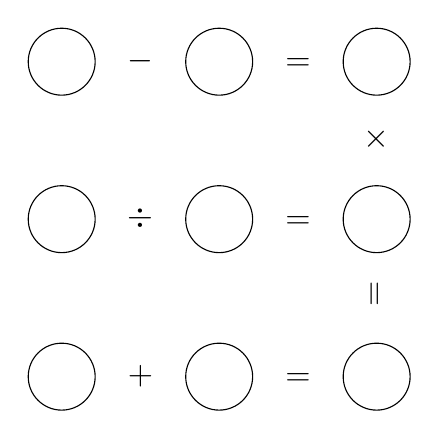
\begin{tikzpicture}
              % Define styles for circles and symbols
              \tikzset{
                circle node/.style={circle, draw, minimum size=0.85cm},
                symbol node/.style={font=\large, text height=1.5ex}
              }

              % First row
              \node[circle node] (c11) at (0,2) {};
              \node[symbol node] (s11) at (1,2) {$-$};
              \node[circle node] (c12) at (2,2) {};
              \node[symbol node] (eq1) at (3,2) {$=$};
              \node[circle node] (c13) at (4,2) {};
              \node[symbol node] (x1) at (4,1) {$\times$};

              % Second row
              \node[circle node] (c21) at (0,0) {};
              \node[symbol node] (s21) at (1,0) {$\div$};
              \node[circle node] (c22) at (2,0) {};
              \node[symbol node] (eq2) at (3,0) {$=$};
              \node[circle node] (c23) at (4,0) {};
              \node[symbol node] (div1) at (4,-1) {\rotatebox{90}{$=$}};

              % Third row
              \node[circle node] (c31) at (0,-2) {};
              \node[symbol node] (s31) at (1,-2) {$+$};
              \node[circle node] (c32) at (2,-2) {};
              \node[symbol node] (eq3) at (3,-2) {$=$};
              \node[circle node] (c33) at (4,-2) {};
            \end{tikzpicture}
        \end{center}
        \Question[3] Find the missing digits in the following multiplication.
        \par\centering
            \begin{tabular}{ccccccc}
                        & & & &$\star$&$\star$&$\star$\\
                $\times$& & & &$\star$&2&$\star$\\
                \hline\\
                        & & & &$\star$&$\star$&$\star$\\
                        & &$\star$&$\star$&$\star$&$\star$&0\\
                        & &$\star$&8&$\star$&0&0\\
                \hline\\
                        &$\star$&$\star$&9&$\star$&2&$\star$\\
                \hline
            \end{tabular}
            \begin{solutionorbox}[2in]
            \end{solutionorbox}
        \Question[3] Use all of the numbers \(1,2,3,4,5,6\) and 7 once and the symbols,\(+,-,\times\) and \(\div\) to make a number sentence that results in 100 .
            \begin{solutionorbox}[2in]
            \end{solutionorbox}
        \Question[4] A fast food store sells nuggets in boxes of 5 and 8 . You can buy 31 nuggets at a time since \(3 \times 5+2 \times 8=31\). What is the largest whole number of nuggets that cannot be purchased?
            \begin{solutionorbox}[2in]
            \end{solutionorbox}
        \Question[4] It is possible to choose four numbers such that any value between 1 and 40 can be made by taking one or more of these numbers and adding or subtracting them from each other. Find the four numbers, and show how the values from 1 to 40 can be made.
            \begin{solutionorbox}[2in]
            \end{solutionorbox}
    \end{questions}
\end{challenge}

    \setcounter{hwmarks}{\thesecmarks}
